\documentclass[tcc,ec]{texfurg} %ppgcomp ou ppgmc

\usepackage[utf8]{inputenc}   % pacote para acentuação, o latin nao funciona.
\usepackage{graphicx} % para inserir figuras
\usepackage{multirow} % tabela"

\title{Modelo TCC para Engenharia de Computação}

\author{UltimoNome}{Nome Sobrenome de}
\advisor[Prof.~Dr.]{Aguiar}{Marilton Sanchotene de}
\coadvisor[Prof.~Dr.]{Gon\c{c}alves}{Eder Mateus Nunes}
\collaborator[Prof.~Dr.]{D'Alessandro}{Andrés Nicolás}

\examiner{Prof.~Dr.~Armando Multas}
\examiner{Prof\textsuperscript{a}.~Dr\textsuperscript{a}.~Nomelinda Longuinha da Silva Paes Netto}
\examiner{Prof.~MSc.~Gerúndio das Dores}


\keyword{Palavra um}
\keyword{Palavra dois}
\keyword{Palavra três}
\keyword{Palavra quatro}
% Até 10 palavras chaves

\begin{document}

%\renewcommand{\advisorname}{Orientadora}           %descomente caso tenhas orientadora
%\renewcommand{\coadvisorname}{Co-orientadora}      %descomente caso tenhas co-orientadora

\maketitle

\sloppy

%Resumo em Português.
\begin{abstract}
     Resumo em Português.
\end{abstract}

\begin{englishabstract}%
  Abstract. In English.
\end{englishabstract}

%Lista de Figuras
\listoffigures

%Lista de Tabelas
\listoftables

%lista de abreviaturas e siglas
\begin{listofabbrv}{SPMD}
		\item[ABC] \textit{Abcd Bcde Cdef}
		\item[XYZ] \textit{Xbcd Ycde Zdef}
       \end{listofabbrv}

%Sumario
\tableofcontents

\chapter{Capítulo Um}

Capítulos podem ter seções e subseções.

%Ex.: Opcional
\section{Seção Um} 

Seção Opcional.

\subsection{Subseção}

Subseção Opcional.

\chapter{Capítulo Dois}

Conceitos e trabalhos que estão relacionados ao projeto.

Exemplos de citação. 

Bla bla bla bla bla bla bla bla bla
bla bla bla bla bla bla bla bla bla bla bla bla bla bla bla bla bla
bla bla bla bla bla bla bla bla bla bla bla bla bla bla bla bla
bla bla bla bla bla bla bla bla bla bla bla bla
\citep{knuth:84}.

\citet{boulic:91} apresentou o conceito de bla bla bla bla bla bla bla
bla bla bla bla bla bla bla bla bla bla bla bla bla bla bla bla bla
bla bla bla bla bla bla bla bla bla bla bla bla bla bla bla bla
bla bla bla bla bla bla bla bla bla bla bla bla bla bla bla bla bla
bla bla bla bla bla bla bla bla bla bla bla bla bla bla bla bla bla
bla bla.

 Bla bla bla bla bla bla bla bla bla
bla bla bla bla bla bla bla bla bla bla bla bla bla bla bla bla bla
bla bla bla bla bla bla bla bla bla bla bla bla bla bla bla bla
bla bla bla bla bla bla bla bla bla bla bla bla
\citep{knuth:84, smith:99}.


\chapter{Capítulo Três}


Exemplo de figura. A figura~\ref{nome_figura} apresenta bla bla bla.

      \begin{figure}[htbp]
        \centering 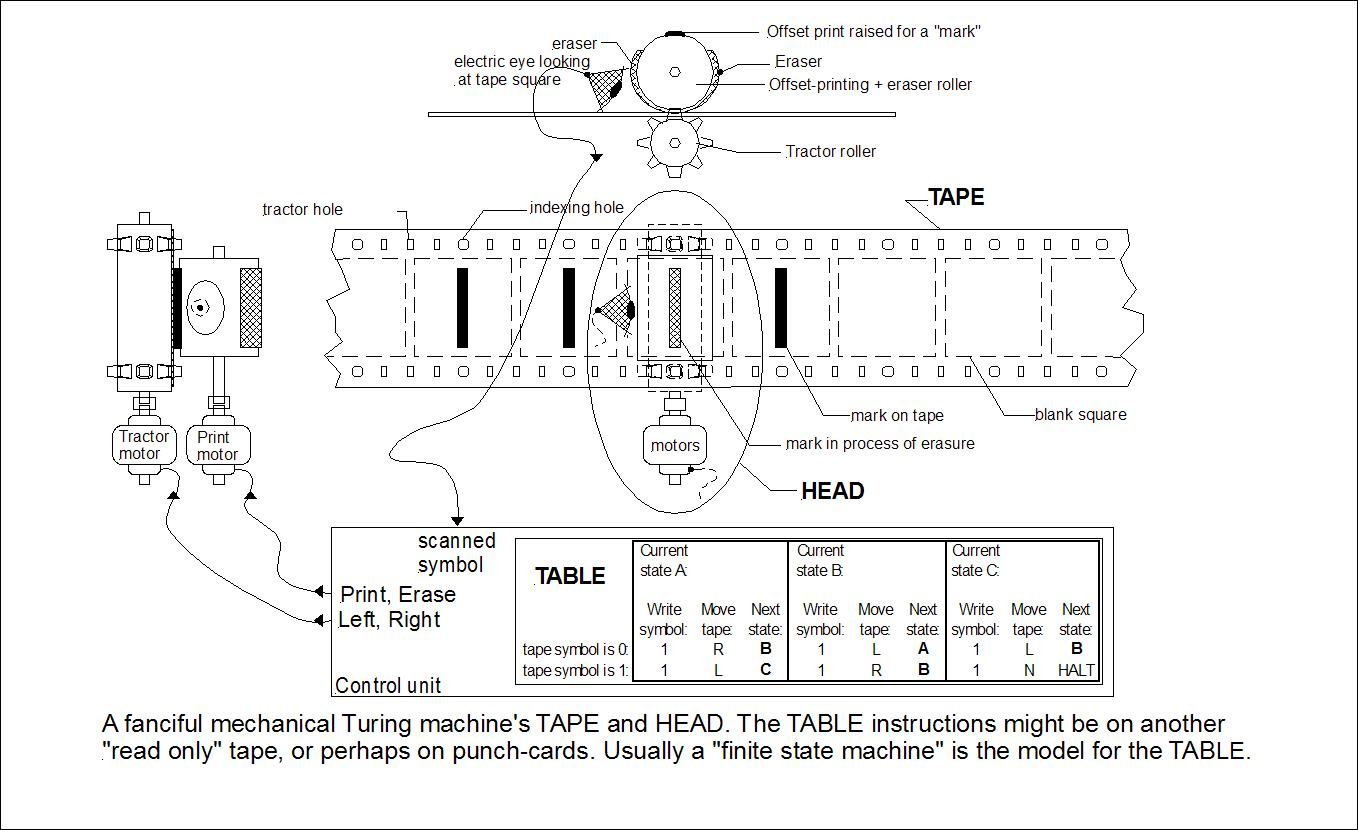
\includegraphics[scale=.3]{turing_machine.eps}
        \caption{Legenda de Figura}
        \label{nome_figura}
    \end{figure}

\chapter{Capítulo Quatro}

Exemplo de Tabela. Conforme tabela~\ref{tabela}, bla bla bla.

\begin{table}[htbp]
\begin{center}
\caption{Nome da Tabela}
\label{tabela}
\begin{tabular}{ccc}
\hline
Blabla & Blabla & Blablabla\\
\hline
1 & 2  & 3 \\
4 & 5  & 6 \\
7 & 8  & 9 \\
10 & 11  & 12 \\
\hline
\end{tabular}
\end{center}
\end{table}


\bibliography{bibliografia}
\bibliographystyle{abnt}

% Anexos (Opcional)
\annex
\chapter{Um Anexo}

  Bla blabla blablabla bla.  Bla blabla blablabla bla.  Bla blabla blablabla
  bla.  Bla blabla blablabla bla.  Bla blabla blablabla bla.  Bla blabla
  blablabla bla.  Bla blabla blablabla bla.  Bla blabla blablabla bla.  Bla
  blabla blablabla bla.  Bla blabla blablabla bla.  Bla blabla blablabla bla.
  Bla blabla blablabla bla.  Bla blabla blablabla bla.  Bla blabla blablabla
  bla.  Bla blabla blablabla bla.  Bla blabla blablabla bla.  Bla blabla
  blablabla bla.  Bla blabla blablabla bla.  Bla blabla blablabla bla.  Bla
  blabla blablabla bla.  Bla blabla blablabla bla.

  Bla blabla blablabla bla.  Bla blabla blablabla bla.  Bla blabla blablabla
  bla.  Bla blabla blablabla bla.  Bla blabla blablabla bla.  Bla blabla
  blablabla bla.  Bla blabla blablabla bla.  Bla blabla blablabla bla.  Bla
  blabla blablabla bla.  Bla blabla blablabla bla.  Bla blabla blablabla bla.
  Bla blabla blablabla bla.  Bla blabla blablabla bla.  Bla blabla blablabla
  bla.  Bla blabla blablabla bla.  Bla blabla blablabla bla.  Bla blabla
  blablabla bla.  Bla blabla blablabla bla.  Bla blabla blablabla bla.  Bla
  blabla blablabla bla.  Bla blabla blablabla bla.

\chapter{Outro Anexo}

  Bla blabla blablabla bla.  Bla blabla blablabla bla.  Bla blabla blablabla
  bla.  Bla blabla blablabla bla.  Bla blabla blablabla bla.  Bla blabla
  blablabla bla.  Bla blabla blablabla bla.  Bla blabla blablabla bla.  Bla
  blabla blablabla bla.  Bla blabla blablabla bla.  Bla blabla blablabla bla.
  Bla blabla blablabla bla.  Bla blabla blablabla bla.  Bla blabla blablabla
  bla.  Bla blabla blablabla bla.  Bla blabla blablabla bla.  Bla blabla
  blablabla bla.  Bla blabla blablabla bla.  Bla blabla blablabla bla.  Bla
  blabla blablabla bla.  Bla blabla blablabla bla.

  Bla blabla blablabla bla.  Bla blabla blablabla bla.  Bla blabla blablabla
  bla.  Bla blabla blablabla bla.  Bla blabla blablabla bla.  Bla blabla
  blablabla bla.  Bla blabla blablabla bla.  Bla blabla blablabla bla.  Bla
  blabla blablabla bla.  Bla blabla blablabla bla.  Bla blabla blablabla bla.
  Bla blabla blablabla bla.  Bla blabla blablabla bla.  Bla blabla blablabla
  bla.  Bla blabla blablabla bla.  Bla blabla blablabla bla.  Bla blabla
  blablabla bla.  Bla blabla blablabla bla.  Bla blabla blablabla bla.  Bla
  blabla blablabla bla.  Bla blabla blablabla bla.

\end{document}